% Tracking and Amplifying Linguistic Ambiguity in LLM-Generated Connections Puzzles
%
% Compile with the official ACL style files (https://github.com/acl-org/acl-style-files):
% place acl.sty in this directory, then: pdflatex main && bibtex main && pdflatex main && pdflatex main
% On Overleaf: upload this folder plus acl.sty.
\documentclass[11pt]{article}
\usepackage[review]{acl}   % switch to [final] for camera-ready
\usepackage{times}
\usepackage{latexsym}
\usepackage{graphicx}
\usepackage{booktabs}
\usepackage{amsmath}
\usepackage{tikz}
\usetikzlibrary{arrows.meta,positioning}
\usepackage{enumitem}

\title{Tracking and Amplifying Linguistic Ambiguity in\\ LLM-Generated Connections Puzzles}

\author{Anonymous Submission}

\begin{document}
\maketitle

\begin{abstract}
The New York Times' \emph{Connections} puzzle asks players to partition sixteen words into four themed groups, and derives much of its difficulty from linguistic ambiguity: words that could plausibly belong to several groups. We present a framework for \emph{generating} Connections-style puzzles with controlled, amplified ambiguity. We (i) define a taxonomy of five ambiguity types (polysemy, homonymy, idiomatic, syntactic, and figurative); (ii) propose a three-stage generation pipeline that combines least-to-most Chain-of-Thought prompting, ReAct-style external validation against WordNet, and Reverse Chain-of-Thought auditing; and (iii) \emph{validate} the embedding-based difficulty metric used to evaluate generated puzzles against ground truth, rather than assuming it. On 422 official NYT puzzles (1,688 groups), intra-group embedding similarity correlates significantly with the official difficulty levels (Spearman $\rho = -0.449$, $p < 10^{-83}$) and orders group pairs within a puzzle correctly 70\% of the time. Groups produced by our pipeline are measurably harder under this validated metric than both real NYT groups and single-prompt GPT-4o groups ($p < 10^{-4}$), and exhibit a clear ambiguity ladder: mean WordNet sense counts rise from 6.1 to 25.0 across the pipeline's four difficulty tiers, while idiomatic multi-word phrases rise from 0\% to 50\%. All prompts, code, data, and every reported number are released for full reproducibility.
\end{abstract}

\section{Introduction}

Word games have tested human linguistic dexterity since antiquity, and they are increasingly used to probe the semantic and abstract reasoning of large language models (LLMs) \citep{todd2024missed, samadarshi2024connecting}. \emph{Connections}, published daily by the New York Times since June 2023, presents a $4\times4$ grid of sixteen words to be partitioned into four groups of four, each sharing a hidden theme. Its difficulty comes less from obscure vocabulary than from \emph{ambiguity}: decoy words that fit several candidate themes, idioms read literally, and homographs whose intended sense is revealed only by the global solution.

Prior work has studied LLMs as Connections \emph{solvers} \citep{samadarshi2024connecting, todd2024missed} and as \emph{generators} \citep{merino2024making}, but two gaps remain. First, generation work has treated difficulty informally: puzzles are scored by an automatic proxy (typically intra-group embedding similarity) whose agreement with ground-truth difficulty has not itself been measured. An unvalidated evaluator cannot validate a generator. Second, ambiguity---the mechanism that actually makes these puzzles hard---has not been given an explicit, linguistically grounded treatment that a generation method can target and an evaluation method can track.

We address both gaps. Our contributions are:

\begin{itemize}[leftmargin=*, itemsep=1pt, topsep=2pt]
    \item \textbf{A taxonomy of linguistic ambiguity for word puzzles} (\S\ref{sec:taxonomy}) covering polysemy, homonymy, idiomatic, syntactic, and figurative ambiguity, with an operationalization in WordNet \citep{miller1995wordnet}.
    \item \textbf{A three-stage generation pipeline} (\S\ref{sec:pipeline}) that amplifies ambiguity by construction: least-to-most Chain-of-Thought generation of four groups with escalating ambiguity \citep{zhou2023least, wei2022chain}, ReAct-style external validation against WordNet \citep{yao2023react}, and Reverse Chain-of-Thought auditing \citep{xue2023rcot}. All prompts are given verbatim in Appendix~\ref{app:prompts}.
    \item \textbf{A validation of the difficulty metric itself} (\S\ref{sec:validation}): on 422 official NYT puzzles with ground-truth difficulty levels, mean intra-group embedding similarity correlates with official difficulty at $\rho=-0.449$ ($p<10^{-83}$) and achieves 70\% pairwise ordering accuracy within puzzles---validating the metric as a coarse difficulty signal while quantifying its limits.
    \item \textbf{A corpus-level analysis} (\S\ref{sec:results}) showing that the pipeline realizes the intended ambiguity ladder (mean sense counts 6.1$\rightarrow$25.0; idiomatic phrase ratio 0$\rightarrow$0.5 across tiers) and produces groups that are harder under the validated metric than real NYT groups and single-prompt GPT-4o baselines.
    \item \textbf{A complete, released experimental stack}: generation pipeline, metrics, figures, datasets, and a documented solver-evaluation harness, so that every number in this paper can be regenerated from a single repository.
\end{itemize}

\section{Related Work}

\paragraph{Connections and LLMs.}
\citet{merino2024making} use GPT-4 to generate novel Connections puzzles and evaluate them with human playtests; \citet{todd2024missed} frame Connections as a benchmark of lateral thinking for LLM solvers; and \citet{samadarshi2024connecting} evaluate both LLMs and humans as solvers, finding that even strong models trail expert players substantially. We complement this line by making the \emph{ambiguity} of generated puzzles an explicit, controllable, and measurable objective, and by validating the automatic difficulty measure that generation studies rely on.

\paragraph{Reasoning frameworks.}
Chain-of-Thought prompting elicits intermediate reasoning steps \citep{wei2022chain}; least-to-most prompting decomposes tasks into progressively harder subproblems \citep{zhou2023least}; ReAct interleaves reasoning with calls to external tools \citep{yao2023react}; Tree of Thoughts explores and evaluates alternative reasoning branches \citep{yao2023tree}; and Reverse Chain-of-Thought reconstructs a problem from a candidate solution to detect inconsistencies \citep{xue2023rcot}. Recent analyses caution that apparent reasoning gains can be brittle under surface perturbations \citep{mirzadeh2024gsm}, reinforcing the need for external, non-LLM validation---which motivates the WordNet-based stage of our pipeline.

\paragraph{Procedural content generation.}
LLM-based PCG has produced playable levels and game content in other domains \citep{sudhakaran2023mariogpt}. Word-puzzle generation is a natural PCG target because validity constraints are discrete and checkable; we make those constraints explicit (\S\ref{sec:constraints}) and enforce a subset automatically.

\paragraph{Lexical ambiguity.}
Our taxonomy draws on classical lexical semantics \citep{cruse1986lexical} and the word-sense disambiguation literature \citep{navigli2009word}, using WordNet sense inventories \citep{miller1995wordnet, fellbaum1998wordnet} as an operational proxy for ambiguity.

\section{A Taxonomy of Ambiguity in Word Puzzles}
\label{sec:taxonomy}

We distinguish five ambiguity types, chosen because each corresponds to a distinct mechanism by which a Connections group can mislead a solver:

\begin{description}[leftmargin=0pt, itemsep=2pt]
    \item[Polysemy.] One lexeme with multiple \emph{related} senses (\emph{bank}: riverbank / financial institution). A polysemous word can anchor two candidate themes simultaneously.
    \item[Homonymy.] Identical form, \emph{unrelated} meanings, often across parts of speech (\emph{bat}: animal / sports equipment). Homonyms support decoy groups whose theme applies to the unintended sense.
    \item[Idiomatic.] Multi-word expressions whose meaning is non-compositional (\emph{break the ice}). Literal readings of components create spurious semantic neighbors.
    \item[Syntactic.] Words whose grammatical category is ambiguous in context (\emph{saw} in ``he saw the man with a telescope''), enabling groups defined over a non-obvious reading.
    \item[Figurative.] Metaphorical extensions (\emph{light} as hope). Figurative senses are weakly represented in distributional similarity, making such groups hard for embedding-based solvers and metrics alike.
\end{description}

\paragraph{Operationalization.} For single words we use the WordNet synset inventory: the \emph{sense count} $|\mathrm{syn}(w)|$, sense counts across parts of speech (a heuristic for homonymy), and definition text (a heuristic for figurative senses). Multi-word entries are treated as idiomatic candidates, since WordNet coverage of phrases is sparse. This operationalization is deliberately simple and fully automatic; its limitations are discussed in \S\ref{sec:limitations}.

\section{Puzzle Constraints}
\label{sec:constraints}

The NYT publishes no official construction rules. From an analysis of 422 published puzzles (\S\ref{sec:data}) and the constraints identified by \citet{merino2024making}, we adopt the following necessary conditions for a valid puzzle:

\begin{enumerate}[leftmargin=*, itemsep=1pt, topsep=2pt]
    \item The puzzle contains exactly 16 unique words, partitioned into 4 groups of 4; each word is used exactly once.
    \item Each group's connection applies to all four of its words and to no other word in the puzzle, so the intended solution is unique.
    \item Categories are more specific than surface-form classes such as \textsc{5-letter words}, \textsc{names}, or \textsc{verbs}.
    \item A group's label word does not appear among its members (\emph{green} may not appear in \textsc{shades of green}).
    \item Spelling is contractual: a member fits its category under its printed spelling (\textsc{insect} admits \emph{bee}, not \emph{be}).
    \item The four groups span an intended difficulty gradient (the NYT's yellow $<$ green $<$ blue $<$ purple).
\end{enumerate}

Conditions 1 and the group-shape part of 2 are checked automatically by our pipeline; the remaining conditions are targeted by prompting and audited in the verification stage. This list consolidates the ten partially redundant criteria of an earlier version of this work into six non-overlapping conditions.

\section{Ambiguity-Amplifying Generation Pipeline}
\label{sec:pipeline}

\begin{figure}[t]
\centering
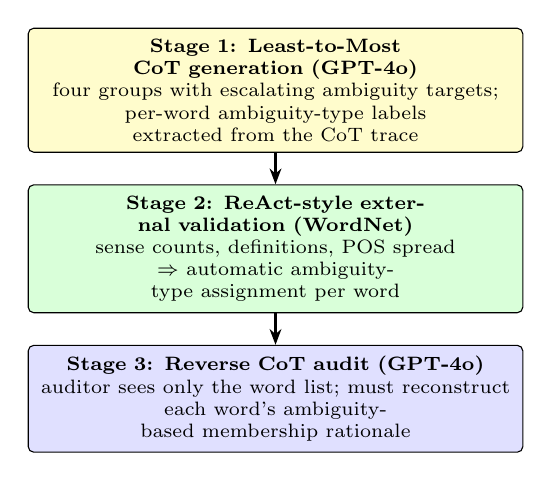
\begin{tikzpicture}[
    node distance=4mm,
    stage/.style={draw, rounded corners=2pt, align=center, font=\scriptsize, inner sep=4pt, text width=60mm},
    arr/.style={-{Stealth[length=2mm]}, thick}
]
\node[stage, fill=yellow!20] (s1) {\textbf{Stage 1: Least-to-Most CoT generation (GPT-4o)}\\ four groups with escalating ambiguity targets;\\ per-word ambiguity-type labels extracted from the CoT trace};
\node[stage, fill=green!15, below=of s1] (s2) {\textbf{Stage 2: ReAct-style external validation (WordNet)}\\ sense counts, definitions, POS spread\\ $\Rightarrow$ automatic ambiguity-type assignment per word};
\node[stage, fill=blue!12, below=of s2] (s3) {\textbf{Stage 3: Reverse CoT audit (GPT-4o)}\\ auditor sees only the word list; must reconstruct\\ each word's ambiguity-based membership rationale};
\draw[arr] (s1) -- (s2);
\draw[arr] (s2) -- (s3);
\end{tikzpicture}
\caption{The three-stage generation pipeline. Every stage writes a JSON artifact that is released with the paper; prompts are reproduced verbatim in Appendix~\ref{app:prompts}.}
\label{fig:pipeline}
\end{figure}

Figure~\ref{fig:pipeline} summarizes the pipeline. Each puzzle is generated group-by-group with an explicit ambiguity ladder, then validated externally, then audited in reverse.

\subsection{Stage 1: Least-to-Most CoT Generation}
Following least-to-most prompting \citep{zhou2023least}, the four groups are requested in order of increasing ambiguity: (1) a clearly defined semantic category; (2) a category with overlapping, flexible membership; (3) words chosen for polysemy or homonymy; (4) items exhibiting idiomatic, syntactic, or figurative ambiguity. The model (GPT-4o, temperature 0.7) produces step-by-step reasoning naming the ambiguity type of every word, then a machine-parseable list. A rule-based extractor recovers the word list and the self-declared ambiguity labels from the trace.

\subsection{Stage 2: ReAct-Style External Validation}
LLM self-assessments of ambiguity are unreliable \citep{mirzadeh2024gsm}, so Stage 2 grounds each word in an external resource in the spirit of ReAct's tool calls \citep{yao2023react}: WordNet supplies the number of senses, up to five definitions, and the part-of-speech spread of each word. From these, an ambiguity type is assigned deterministically (multi-word $\Rightarrow$ idiomatic candidate; senses spanning POS $\Rightarrow$ homonymy; metaphor-marked glosses $\Rightarrow$ figurative; otherwise polysemy). Stage 2 is entirely LLM-free, providing a check that does not share the generator's failure modes.

\subsection{Stage 3: Reverse CoT Audit}
Inspired by RCoT \citep{xue2023rcot}, an auditor model receives \emph{only} the final word list---not the generation rationale---and must justify each word's membership in terms of the taxonomy. Groups whose audit fails to recover a coherent ambiguity-based rationale are flagged. This inverts the generation direction, catching groups that were accepted on the strength of a persuasive but unfaithful generation trace.

\subsection{Released corpus}
Running the pipeline for 50 puzzles (200 groups, 800 words/phrases) produced the corpus analyzed in \S\ref{sec:results}; all stage-wise artifacts (prompts, raw responses, extracted lists, WordNet records, audit traces) are included in the repository.

\section{Measuring Difficulty---and Validating the Measure}
\label{sec:validation}

\subsection{Metric}
For a group $G=\{w_1,\dots,w_n\}$ we define difficulty via mean pairwise similarity over the $\binom{n}{2}$ distinct pairs:
\begin{equation}
D(G) = \binom{n}{2}^{-1} \sum_{i<j} \cos\!\big(e(w_i),\, e(w_j)\big),
\label{eq:difficulty}
\end{equation}
where $e(\cdot)$ is a sentence-embedding function (all-mpnet-base-v2; \citealp{reimers2019sentence}). Lower similarity means the group's members are semantically farther apart, hence harder to recognize as a group. (An earlier version of this work averaged over all $n^2$ ordered pairs including self-similarity, which compresses the scale; Eq.~\ref{eq:difficulty} uses distinct pairs only.)

\subsection{Ground-truth validation}
\label{sec:data}
An automatic generator evaluated only by an automatic metric is circular unless the metric is itself validated. We therefore test $D$ against ground truth: the NYT assigns every published group a difficulty level 0--3 (yellow, green, blue, purple). Our evaluation corpus contains 422 official puzzles (June 2023 onward; 1,688 groups), obtained from the community-maintained NYT-Connections-Answers archive\footnote{\url{https://github.com/Eyefyre/NYT-Connections-Answers}} and redistributed in the repository as \texttt{Real\_Data.json} / \texttt{Real\_Data\_Ans.json}; puzzle words and solutions are facts about the published games, used here for non-commercial research.

\begin{figure}[t]
\centering
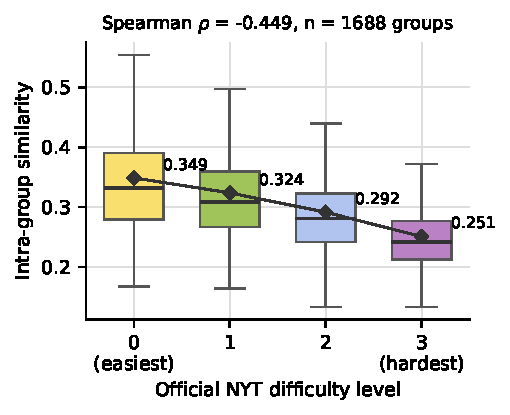
\includegraphics[width=\columnwidth]{figures/metric_validation.pdf}
\caption{Intra-group embedding similarity (Eq.~\ref{eq:difficulty}) against official NYT difficulty levels for 1,688 groups from 422 puzzles. Similarity decreases monotonically with official difficulty.}
\label{fig:validation}
\end{figure}

\begin{table}[t]
\centering\small
\begin{tabular}{lcc}
\toprule
\textbf{Official level} & \textbf{Mean $D(G)$} & $n$ \\
\midrule
0 (yellow, easiest) & $0.349 \pm 0.102$ & 422 \\
1 (green)           & $0.324 \pm 0.089$ & 422 \\
2 (blue)            & $0.292 \pm 0.081$ & 422 \\
3 (purple, hardest) & $0.251 \pm 0.067$ & 422 \\
\midrule
Spearman $\rho$ (level, $D$) & \multicolumn{2}{c}{$-0.449$ ($p < 10^{-83}$)} \\
Pairwise ordering acc. & \multicolumn{2}{c}{$0.700$ (1{,}769/2{,}526)} \\
\bottomrule
\end{tabular}
\caption{Validation of the difficulty metric against ground-truth NYT levels. Ordering accuracy: fraction of within-puzzle group pairs with distinct official levels that the metric ranks in the official order (chance $=0.5$).}
\label{tab:validation}
\end{table}

Table~\ref{tab:validation} and Figure~\ref{fig:validation} show the result. Mean similarity decreases monotonically across all four official levels; the group-level Spearman correlation is $\rho=-0.449$ ($p<10^{-83}$), and within puzzles the metric orders 70.0\% of comparable group pairs in agreement with the NYT's own ordering (chance 50\%).

\paragraph{Interpretation.} The metric is a real but \emph{coarse} difficulty signal: it reliably separates the easiest from the hardest tiers yet misorders 30\% of adjacent pairs. Inspection of failures shows they concentrate in wordplay categories (e.g., ``\_\_\_ + fish'' completions or palindromes) whose difficulty is orthogonal to semantic diversity. We therefore treat $D$ as evidence of relative hardness at corpus level, not as a per-puzzle oracle, and we complement it with the ambiguity measures of \S\ref{sec:results}. This addresses directly the circularity concern raised against automatic-generation-plus-automatic-evaluation designs.

\section{Results}
\label{sec:results}

\subsection{Does the pipeline realize the ambiguity ladder?}

\begin{figure}[t]
\centering
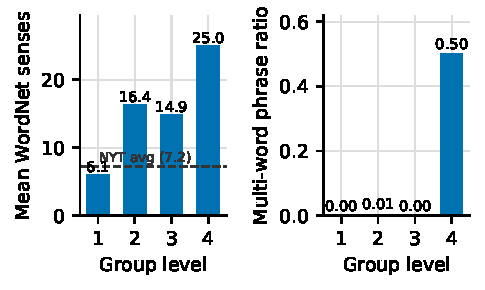
\includegraphics[width=\columnwidth]{figures/ambiguity_ladder.pdf}
\caption{Ambiguity by pipeline tier over 50 generated puzzles: mean WordNet sense count of single-word members (left; dashed line: real NYT average) and fraction of multi-word idiomatic phrases (right).}
\label{fig:ladder}
\end{figure}

\begin{table}[t]
\centering\small
\setlength{\tabcolsep}{4.2pt}
\begin{tabular}{lcccc}
\toprule
\textbf{Tier} & \textbf{Senses} & \textbf{Ambig.\ ratio} & \textbf{$\geq$5 senses} & \textbf{Phrases} \\
\midrule
1 & 6.1  & 0.86 & 0.58 & 0.00 \\
2 & 16.4 & 1.00 & 0.98 & 0.01 \\
3 & 14.9 & 1.00 & 0.98 & 0.00 \\
4 & 25.0 & 0.92 & 0.92 & 0.50 \\
\midrule
NYT & 7.4 & 0.85 & 0.56 & 0.01 \\
\bottomrule
\end{tabular}
\caption{Ambiguity metrics by pipeline tier (50 groups per tier) vs.\ all real NYT groups (1,688). \emph{Senses}: mean WordNet sense count of single-word members. \emph{Ambig.\ ratio}: fraction with $\geq 2$ senses. \emph{Phrases}: fraction of multi-word members.}
\label{tab:ladder}
\end{table}

Table~\ref{tab:ladder} and Figure~\ref{fig:ladder} track ambiguity across the four tiers of the 50-puzzle corpus. The intended ladder is realized: tier-1 groups look like real NYT groups (6.1 vs.\ 7.4 mean senses), while tiers 2--4 are far more lexically ambiguous than anything typical of the official game---tier-4 items average 25.0 senses among single words, and half of tier-4 items are multi-word idiomatic expressions, matching that tier's idiomatic/figurative target. The Stage-2 typology shifts accordingly, from homonymy/polysemy-dominated tiers 2--3 to an idiom-heavy tier 4. Tiers 2 and 3 are statistically indistinguishable in sense count, an honest signal that ``flexible category'' and ``polysemy/homonymy'' prompts recruit similar vocabulary; collapsing them is a candidate simplification.

Notably, in the \emph{real} game, mean sense counts are flat across official levels (7.5, 8.1, 7.8, 6.3 for levels 0--3): NYT difficulty is driven by cross-group interaction and wordplay rather than lexical ambiguity of members. Lexical ambiguity is thus a \emph{new} difficulty axis that generated puzzles can push far beyond the official distribution.

\subsection{Are pipeline groups harder under the validated metric?}

\begin{figure}[t]
\centering
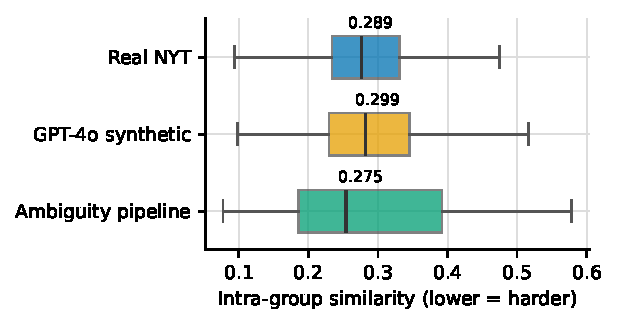
\includegraphics[width=\columnwidth]{figures/dataset_comparison.pdf}
\caption{Distribution of intra-group similarity by source. Lower = harder under the validated metric.}
\label{fig:comparison}
\end{figure}

\begin{table}[t]
\centering\small
\begin{tabular}{lccc}
\toprule
\textbf{Source} & $n$ & \textbf{Mean $D(G)$} & $p$ vs.\ real \\
\midrule
Real NYT groups        & 1{,}688 & $0.304 \pm 0.093$ & --- \\
GPT-4o single-prompt   & 6{,}016 & $0.299 \pm 0.097$ & $6.0\times10^{-3}$ \\
Ambiguity pipeline     & 200     & $0.275 \pm 0.126$ & $1.0\times10^{-5}$ \\
\bottomrule
\end{tabular}
\caption{Intra-group similarity by source (Mann--Whitney $U$ vs.\ real NYT groups). The single-prompt baseline is the 2,000-puzzle GPT-4o synthetic set generated without the ambiguity pipeline.}
\label{tab:comparison}
\end{table}

Table~\ref{tab:comparison} and Figure~\ref{fig:comparison} compare three sources under Eq.~\ref{eq:difficulty}. Single-prompt GPT-4o puzzles are only marginally more diverse than real ones ($0.299$ vs.\ $0.304$), whereas pipeline groups shift substantially ($0.275$, $p=1.0\times10^{-5}$), with a heavier low-similarity tail (Figure~\ref{fig:comparison}). Combined with Table~\ref{tab:ladder}, this supports the central claim: \emph{explicitly targeting the ambiguity taxonomy, with external validation, produces measurably harder groups than either human construction or naive LLM generation}---as measured by a metric whose relationship to ground-truth difficulty we quantified rather than assumed.

\section{Solver Evaluation Protocol}
\label{sec:solver}

Difficulty for \emph{machine} solvers is the natural third axis. The repository releases a complete solver harness (\texttt{experiments/solve\_puzzles.py}) that evaluates any OpenAI-compatible chat model on real or generated puzzles under three fully specified prompting strategies---direct, Chain-of-Thought, and Tree-of-Thoughts \citep{wei2022chain, yao2023tree}; prompts in Appendix~\ref{app:prompts}---and reports puzzle solve rate (all four groups exact), group accuracy (partial credit), and per-official-level accuracy with per-instance logs. We deliberately report no solver numbers here: solve-rate figures from an earlier version of this work were not regenerable from a specified protocol, and we consider unreproducible numbers worse than absent ones. The harness makes the experiment a single documented command, and human-subject evaluation of solvability and enjoyment (protocol in Appendix~\ref{app:human}) is the necessary companion study.

\section{Conclusion}

We reframed Connections puzzle generation around its core difficulty mechanism---linguistic ambiguity---via a five-type taxonomy, a generate-validate-audit pipeline that amplifies ambiguity by construction, and, critically, a ground-truth validation of the embedding-based difficulty metric that generation studies in this space rely on. The validated metric ($\rho=-0.449$; 70\% pairwise ordering accuracy on 422 official puzzles) shows pipeline-generated groups to be harder than both real and naively generated ones, and WordNet-based measures confirm the pipeline's ambiguity ladder is realized in the output. Beyond Connections, the pattern---\emph{taxonomize the difficulty mechanism, generate against it, validate the evaluator}---applies to procedural generation of word games generally.

\section{Limitations}
\label{sec:limitations}

\textbf{No human evaluation yet.} All evaluation is automatic. The difficulty metric is validated against NYT editorial levels, which encode the editors' intent rather than measured human solve behavior, and no property akin to ``fun'' or ``fairness'' is measured; a group can be diverse yet unsolvable. Appendix~\ref{app:human} specifies the human study this work requires before any claim about player experience.
\textbf{Metric coarseness.} The validated correlation is moderate ($\rho=-0.449$); 30\% of within-puzzle orderings disagree with ground truth, concentrated in wordplay categories. Corpus-level comparisons are supported; per-puzzle difficulty certification is not.
\textbf{WordNet as ambiguity oracle.} Sense counts conflate polysemy with homonymy, under-represent idioms, and miss proper-noun senses (e.g., \emph{Jordan} as country vs.\ athlete), and the homonymy/figurative heuristics of Stage 2 are simple. \textbf{Pipeline scope.} Stage 3 audits groups independently; cross-group decoy structure---a hallmark of expert NYT construction---is not yet explicitly optimized. \textbf{Single generator family.} Generation used GPT-4o; generality across model families is untested. \textbf{Puzzle-type coverage.} Purely orthographic categories (palindromes, hidden words) fall outside a semantic-ambiguity taxonomy and are correspondingly outside the pipeline's current reach.

\section*{Ethics Statement}
Puzzle words and solutions from the published NYT game are used as facts about published works for non-commercial research, via a public community archive; no NYT text beyond category labels and words is redistributed. Generated puzzles are marked as machine-generated. The proposed human study (Appendix~\ref{app:human}) involves minimal-risk gameplay with informed consent and no collection of sensitive data.

\bibliography{refs}

\appendix

\section{Prompts (verbatim)}
\label{app:prompts}

All prompts are stored as versioned text files under \texttt{prompts/} in the repository and reproduced here verbatim.

\subsection{Stage 1 system prompt}
\begin{quote}\small\ttfamily
You are an expert puzzle designer specializing in linguistic ambiguity. Always provide a complete Python list as requested.
\end{quote}

\subsection{Stage 1 user prompts (tiers 1--4)}
Each tier prompt shares the frame:
\begin{quote}\small\ttfamily
You are creating a Connections-style puzzle. Each group must contain exactly 4 related words or phrases.\\[2pt]
\textrm{[tier-specific task, below]}\\[2pt]
Explain your reasoning step by step, specifying the ambiguity type (polysemy, homonymy, idiomatic, syntactic, figurative) for each word or phrase. At the end, provide the 4 final words/phrases as a Python list in the format: ['word1', 'word2', 'word3', 'word4']. Ensure the list is complete and correctly formatted.
\end{quote}

Tier-specific tasks:
\begin{quote}\small\ttfamily
\textbf{Tier 1:} Group 1: Choose 4 words that belong to a clearly defined semantic category (e.g., colors: red, blue, green, yellow).\\[3pt]
\textbf{Tier 2:} Group 2: Choose 4 words with slightly overlapping or flexible meanings (e.g., tools: hammer, saw, drill, wrench).\\[3pt]
\textbf{Tier 3:} Group 3: Choose 4 words that exhibit polysemy (multiple related senses, e.g., 'bank' as riverbank or financial institution) or homonymy (same spelling/pronunciation, distinct meanings, e.g., 'bat' as animal or sports equipment).\\[3pt]
\textbf{Tier 4:} Group 4: Choose 4 words or phrases that exhibit idiomatic ambiguity (phrases with non-literal meanings, e.g., 'break the ice'), syntactic ambiguity (words that create ambiguous sentence structures, e.g., 'saw' in 'he saw the man with a telescope'), or figurative ambiguity (metaphorical meanings, e.g., 'light' as brightness or metaphorical hope).
\end{quote}

\subsection{Stage 3 (RCoT) prompts}
System:
\begin{quote}\small\ttfamily
You are a puzzle auditor verifying semantic ambiguity per a defined taxonomy.
\end{quote}
User template (\texttt{\{word\_list\}} substituted):
\begin{quote}\small\ttfamily
You are verifying a word puzzle group. The group contains the following words or phrases:\\
\{word\_list\}\\[2pt]
For each word or phrase, explain why it belongs in the group, focusing on its ambiguity type (polysemy, homonymy, idiomatic, syntactic, figurative). Describe how its multiple meanings or interpretations relate to the theme of ambiguity.
\end{quote}

\subsection{Solver prompts}
The direct, CoT, and ToT solver prompts used by the released harness are in \texttt{prompts/solver\_direct.txt}, \texttt{prompts/solver\_cot.txt}, and \texttt{prompts/solver\_tot.txt}; the ToT prompt explores three complete candidate partitions (literal-semantic, wordplay-first, decoy-averse), scores each against the validity constraints of \S\ref{sec:constraints}, and selects or backtracks.

\section{Dataset details}
\label{app:data}

\textbf{Real puzzles.} 422 official puzzles (2023-06-12 onward), 1,688 groups, with per-group official difficulty levels 0--3, from the public NYT-Connections-Answers archive (see \S\ref{sec:data}). \textbf{Single-prompt synthetic set.} 2,000 training / 400 test puzzles generated with GPT-4o from a single prompt without the ambiguity pipeline (6,016 unique parsed groups after deduplication and cleaning). \textbf{Pipeline corpus.} 50 puzzles $\times$ 4 tiers with all stage-wise artifacts. Exact file formats and regeneration commands are documented in the repository README.

\section{Human evaluation protocol (designed, not yet run)}
\label{app:human}

\textbf{Design.} Within-subjects, three conditions (real NYT / single-prompt GPT-4o / pipeline), 6 puzzles per participant (2 per condition, Latin-square ordered), target $n \geq 30$ fluent English speakers recruited on a crowdsourcing platform with a standard Connections interface (four guesses allowed, one-away feedback). \textbf{Measures.} Solve rate, groups solved, time-to-solve, error count (behavioral); post-puzzle 7-point ratings of difficulty, fairness (``the intended groupings felt justified once revealed''), and enjoyment; a forced-choice ``would you play another like this?''. \textbf{Analyses.} Mixed-effects models with participant and puzzle random effects; the pre-registered primary hypotheses are (H1) behavioral difficulty ordering pipeline $>$ single-prompt $>$ real, (H2) $D(G)$ predicts behavioral solve rate at the group level, (H3) pipeline puzzles remain within one point of real puzzles on fairness. H3 is the safeguard against the failure mode where amplified ambiguity yields unsolvable or arbitrary puzzles.

\end{document}
